\documentclass[conference]{IEEEtran}

% =========================================================
% PACKAGES
% =========================================================
\usepackage[T1]{fontenc}
\usepackage{cite}
\usepackage{amsmath,amssymb,amsfonts}
\usepackage{graphicx}
\usepackage{xcolor}
\usepackage{booktabs}
\usepackage{multirow}
\usepackage{array}
\usepackage{url}
\usepackage{balance}
\usepackage{enumitem}

% =========================================================
% PAPER METADATA
% =========================================================
\title{Task-Adaptive Architecture Optimization for LLM-Based Multi-Agent Systems via Reinforcement Learning and Dynamic Graph Construction}

\author{
\IEEEauthorblockN{Naveen Tanikonda}
\IEEEauthorblockA{
Vellore Institute of Technology -- AP\\
naveen.23bce9787@vitapstudent.ac.in
}
\and
\IEEEauthorblockN{VeeraBhadra Jagarlamudi}
\IEEEauthorblockA{
Vellore Institute of Technology -- AP\\
bhadra.23bce9780@vitapstudent.ac.in
}
\and
\IEEEauthorblockN{Sriram Somarouthu}
\IEEEauthorblockA{
Vellore Institute of Technology -- AP\\
sriram.23bce20270@vitapstudent.ac.in
}
\and
\IEEEauthorblockN{Ravi Teja Perumalapalli}
\IEEEauthorblockA{
Vellore Institute of Technology -- AP\\
teja.23bce9392@vitapstudent.ac.in
}
}

\begin{document}
\maketitle

% =========================================================
% ABSTRACT
% =========================================================
\begin{abstract}
Large Language Model (LLM)-based multi-agent systems coordinate ensembles of specialized agents to solve complex reasoning, coding, and information retrieval tasks. However, conventional multi-agent frameworks typically deploy rigid, monolithic static topologies, enforcing identical agent configurations across heterogeneous tasks. This static paradigm incurs substantial computational redundancy, unnecessary communication overhead, prolonged sequential latency, and inflated inference costs for simple queries. In this paper, we investigate a task-adaptive architecture optimization framework for LLM-based multi-agent systems, where agent activations, operational roles, and directed communication topologies are dynamically tailored to input task requirements. We formulate the multi-agent topology selection problem as a Markov Decision Process (MDP) and present two clearly demarcated contributions. First, as our primary live runtime contribution (C2), we implement an active tabular Q-learning selector coupled with an invariant-checked architecture manager and a dynamic LangGraph compilation engine. Across an 18-task benchmark suite spanning six functional domains, the runtime Q-learning adapter achieves a 36.19\% net token reduction ($p = 9.85 \times 10^{-10}$), a 50.0\% active agent pruning rate relative to a 6-agent roster (40.0\% relative to a 5-agent baseline), and compresses the sequential critical execution path from 5.0 to 2.89 hops, while preserving 100\% capability coverage across 16 of 18 tasks (94.44\% macro mean) with sub-15\,ms dynamic compilation latency. Second, as an experimental exploration (C1), we investigate task-conditioned cross-task neural adaptation using a shared policy trained across task environments and evaluated on held-out tasks. We rigorously document empirical boundaries: under a discrete action space restricted to planning and analysis, neural adaptation plateaus at zero gain on four tasks due to missing domain-specific roles, while exhibiting protective stability on summarization. Our findings provide reproducible empirical evidence and architectural principles for deploying parsimonious, dynamically compiled multi-agent workflows.
\end{abstract}

\begin{IEEEkeywords}
Multi-agent systems, large language models, reinforcement learning, adaptive architecture, dynamic workflows, LangGraph, graph pruning, critical path compression.
\end{IEEEkeywords}

% =========================================================
% 1. INTRODUCTION
% =========================================================
\section{Introduction}
\label{sec:introduction}

Large Language Models (LLMs) have demonstrated remarkable efficacy across natural language comprehension, mathematical reasoning, program synthesis, and open-domain problem solving. To overcome the reasoning and context limitations of single-agent prompting, multi-agent systems (MAS) have emerged as the dominant architecture for handling sophisticated decomposition tasks~\cite{hong2024metagpt,lee2026survey,cao2025survey}. In these collaborative architectures, heterogeneous agents assume specialized functional roles---such as planning, information research, code synthesis, critique, and result finalization---communicating through structured control flows.

Despite their empirical success, conventional LLM multi-agent systems suffer from a fundamental architectural limitation: \emph{structural rigidity}. Prevailing frameworks deploy static, predefined execution topologies that invoke the entire multi-agent team regardless of the intrinsic complexity or capability demands of the user request. Under this fixed paradigm, a trivial greeting or direct arithmetic calculation triggers the same heavyweight multi-agent pipeline as an intricate distributed systems design task, executing redundant planning, research, coding, and verification loops. This structural over-provisioning introduces severe practical inefficiencies:
\begin{enumerate}[leftmargin=*]
    \item \textbf{Token Consumption and Financial Cost:} Activating superfluous specialist agents inflates context windows and generates redundant token exchanges, multiplying API costs.
    \item \textbf{Sequential Latency and Execution Bottlenecks:} Linear or densely connected agent pipelines force sequential execution hops, where critical path latency scales with total agent count rather than task difficulty~\cite{Li2025AdaptiveGraphPruning}.
    \item \textbf{Noise Propagation and Hallucination Amplification:} Unnecessary intermediate agent invocations create opportunities for context dilution, drift, and cascading hallucinations~\cite{xiao2026agentdropout}.
\end{enumerate}

To overcome these challenges, recent research has explored dynamic topology optimization, communication graph pruning, and adaptive agent orchestration~\cite{Li2025AdaptiveGraphPruning,Jiang2026GTD,Zhang2025MaAS,wang2026neuralfsm}. However, existing approaches frequently incur substantial search overhead (e.g., multi-round deliberation in DyLAN~\cite{liu2026llm} or evolutionary population rollouts in MaAS~\cite{Zhang2025MaAS}), which can consume thousands of tokens before task execution commences.

In this work, we investigate task-adaptive architecture optimization for LLM-based multi-agent systems via reinforcement learning and dynamic workflow compilation. We decouple the research into two distinct contributions that must remain strictly delineated:

\textbf{Contribution 1 (C1: Experimental Neural Pathway):} We explore an experimental task-conditioned neural adaptation policy trained across a distribution of task environments and evaluated on held-out tasks. The policy predicts architecture modification scores from concatenated task and state embeddings, optimized via temporal-difference learning. We conduct a rigorous multi-seed evaluation against fresh scratch initialization, deterministic baselines, and random policies. Crucially, we preserve and analyze negative empirical findings, identifying how structural action space restrictions prevent capability recovery. This pathway operates on a deterministic compatibility proxy and does not drive live runtime execution.

\textbf{Contribution 2 (C2: Live Runtime Q-Learning Pipeline):} We implement an operational, end-to-end adaptive runtime system that modifies multi-agent topologies using task-aware tabular Q-learning. Candidate graph mutations (activating/deactivating agents, adding/removing edges, and changing roles) are filtered through a structural validation manager enforcing graph invariants. The validated logical architecture is dynamically converted and compiled into an executable LangGraph StateGraph workflow, supporting conditional routing and quality rework.

We formulate three central research questions:
\begin{itemize}[leftmargin=*]
    \item \textbf{RQ1 (Topological Efficiency):} Can reinforcement learning prune redundant agents and compress execution critical paths while preserving complete capability coverage?
    \item \textbf{RQ2 (Runtime Compilation Overhead):} Can dynamic multi-agent graph construction and compilation be executed with negligible latency overhead relative to LLM inference?
    \item \textbf{RQ3 (Cross-Task Knowledge Transfer):} Does cross-task pretraining of a neural policy provide measurable adaptation advantages over training from scratch on unseen tasks?
\end{itemize}

The remainder of this paper is organized as follows. Section~\ref{sec:related_work} reviews related literature. Section~\ref{sec:problem_formulation} establishes the formal problem definition and evaluation metrics. Section~\ref{sec:architecture} presents the proposed system architecture. Section~\ref{sec:neural_adaptation} details the experimental neural adaptation pathway (C1). Section~\ref{sec:runtime_q_learning} details the runtime Q-learning and dynamic LangGraph pipeline (C2). Section~\ref{sec:experimental_setup} outlines the benchmark suite and evaluation setup. Section~\ref{sec:experimental_results} presents quantitative empirical results. Section~\ref{sec:statistical_analysis} provides inferential statistical analysis. Section~\ref{sec:discussion} and Section~\ref{sec:limitations} discuss insights and limitations. Section~\ref{sec:conclusion} concludes the paper.

% =========================================================
% 2. RELATED WORK
% =========================================================
\section{Related Work}
\label{sec:related_work}

\subsection{Static vs. Dynamic LLM-Based Multi-Agent Systems}
Multi-agent collaboration frameworks coordinate ensembles of specialized LLMs to tackle sophisticated problem decomposition. Foundational architectures such as MetaGPT~\cite{hong2024metagpt}, AutoGen~\cite{wu2023autogen}, and ChatDev~\cite{qian2024chatdev} demonstrated that structuring interactions via Standard Operating Procedures (SOPs) and predefined conversational roles significantly reduces reasoning ambiguity. However, these prevailing systems operate under strict \textit{structural rigidity}: every incoming user query activates the identical monolithic multi-agent pipeline sequentially, regardless of problem complexity. Recent surveys emphasize that static multi-agent pipelines incur severe computational redundancy, inflated inference costs, and latency bottlenecks~\cite{lee2026survey,cao2025survey,sun2024llmmarl}.

To mitigate agent redundancy, AgentDropout~\cite{xiao2026agentdropout} proposed deactivating non-essential agents during multi-turn interactions. Similarly, DyLAN~\cite{liu2024dylan} introduced an unsupervised peer-rating mechanism to filter out low-contributing agents between communication layers, reporting 25--40\% agent pruning and 15--25\% token reductions. However, DyLAN requires all agents to iteratively score their peers at each round, generating an $\mathcal{O}(N^2)$ LLM prompt overhead that negates token efficiency on simple or fast queries.

\subsection{Graph Architecture Search, Optimization, and Pruning}
Transforming multi-agent execution from rigid chains into task-adaptive computation graphs represents an active research frontier. GPTSwarm~\cite{zhuge2024gptswarm} conceptualized LLM ensembles as differentiable computation graphs, using reinforcement learning and policy gradients to optimize edge routing weights. However, GPTSwarm retains a fully connected topological substrate where all agents remain active, focusing on task accuracy (+12.4\% on GAIA) rather than sequential critical-path compression or agent pruning.

AFlow~\cite{zhang2024aflow} investigated automated workflow synthesis by framing agentic code generation as Monte Carlo Tree Search (MCTS), demonstrating that task-adapted workflows surpass static architectures (+5.7\% accuracy). Nevertheless, AFlow requires 15--30 exploratory rollout evaluations per problem, resulting in substantial search latency and token expenditure that prevent instant online query execution. Multi-Agent Architecture Search (MaAS)~\cite{Zhang2025MaAS} introduced agentic supernets to explore role assignments and edge topologies using multi-objective evolutionary algorithms, reporting 18--32\% token savings. Yet, evolutionary search necessitates multi-generation evaluations offline, yielding static architectures per task class rather than dynamic per-query adaptation.

In parallel, Adaptive Graph Pruning (CARD/AGP)~\cite{Li2025AdaptiveGraphPruning} employed contextual bandits to dynamically prune agent communication matrices, compressing critical execution paths by 44\% ($5.0 \to 2.8$ hops). Our proposed AMAS architecture directly connects with and extends these foundations. Rather than incurring multi-round peer deliberation (DyLAN), iterative MCTS rollouts (AFlow), or offline evolutionary generations (MaAS), AMAS couples instant tabular Q-learning action selection ($<1$\,ms decision time, 0 search tokens) with strict invariant validation and compiles the pruned topology directly into an executable LangGraph~\cite{langgraph2024} StateGraph DAG in sub-15\,ms, delivering validated empirical token and latency savings under live LLM execution.

\subsection{Meta-Reinforcement Learning and Cross-Task Transfer}
Meta-RL investigates learning adaptation strategies across task distributions~\cite{Kashikar2025MetaRL,Huang2024AdaptiveMARL}. Contextual meta-MARL has been explored to coordinate heterogeneous agents under varying team attributes~\cite{Huang2024AdaptiveMARL}. Fu et al.~\cite{Fu2026MOFA} investigated mixtures of orthogonal experts for rapid policy transfer. Our experimental neural pathway (C1) explores whether task-conditioned neural policies trained across synthetic task distributions can transfer architectural priors to held-out tasks. We explicitly distinguish this from canonical gradient meta-learning algorithms such as MAML or RL$^2$.

Table~\ref{tab:literature_comparison} provides a systematic comparison between our framework and prominent literature baselines (organized with evaluation dimensions in rows and systems in columns, with AMAS capabilities and empirical bounds bolded).

\begin{table*}[!t]
\centering
\caption{Systematic Comparison with Related Dynamic Multi-Agent Architectures (Features in Rows, Frameworks in Columns)}
\label{tab:literature_comparison}
\footnotesize
\begin{tabular}{lp{2.1cm}p{2.1cm}p{2.1cm}p{2.1cm}p{2.1cm}p{3.2cm}}
\toprule
\textbf{Feature / Dimension} & \textbf{DyLAN}~\cite{liu2024dylan} & \textbf{GPTSwarm}~\cite{zhuge2024gptswarm} & \textbf{AFlow}~\cite{zhang2024aflow} & \textbf{MaAS}~\cite{Zhang2025MaAS} & \textbf{CARD}~\cite{Li2025AdaptiveGraphPruning} & \textbf{AMAS (Ours)} \\
\midrule
\textbf{Adaptation Method} & Peer rating & Graph policy grad. & MCTS rollout & Genetic search & Contextual bandit & \textbf{Q-Learning + Neural Policy} \\
\textbf{Decision Latency} & $\mathcal{O}(N^2)$ LLM calls & Iterative LLM prompts & 15--30 rollouts & Offline evolution & $<10$\,ms routing & \textbf{$<1$\,ms Q-hit (0 tokens)} \\
\textbf{Workflow Compilation} & Layered agent stack & Continuous edge weights & Python code scripts & Static specialist DAG & Routing DAG & \textbf{LangGraph StateGraph DAG} \\
\textbf{Active Agent Pruning} & 25--40\% & None (fixed team) & None (fixed team) & 18--32\% & None (full team) & \textbf{50.0\% (Pool 6) / 40.0\% (Base 5)} \\
\textbf{Critical Path Reduction} & None & None & Variable & None & 44.0\% ($5.0 \to 2.8$) & \textbf{42.2\% ($5.0 \to 2.89$ hops)} \\
\textbf{Empirical Token Savings} & 15--25\% & Negative (utility focus) & Negative (MCTS cost) & 18--32\% & Not reported & \textbf{+60.46\% (Live NIM)} \\
\textbf{Cross-Task Transfer} & No & Task-specific & No & No & Tabular only & \textbf{Evaluated on 5 held-out tasks} \\
\midrule
\textbf{Primary Limitation} & Deliberation token blowup & High training sample cost & Search latency per query & Static offline deployment & Heuristic bandit only & \textbf{Restricted action space ($\Delta Q = 0$ on 3 tasks); under-engineering on cross-domain} \\
\bottomrule
\end{tabular}
\end{table*}


% =========================================================
% 3. PROBLEM FORMULATION
% =========================================================
\section{Problem Formulation}
\label{sec:problem_formulation}

\subsection{Multi-Agent System Representation}
Let the multi-agent system be represented as a directed graph:
\begin{equation}
G = (V, E),
\end{equation}
where $V = \{v_1, v_2, \dots, v_n\}$ denotes the pool of available specialized agent nodes ($n = |V|$), and $E \subseteq V \times V$ represents directed communication and execution control channels. In this study, the master agent roster comprises $n = 6$ potential agent roles:
\begin{equation}
V = \{\text{Planner}, \text{Tool}, \text{Researcher}, \text{Coder}, \text{Critic}, \text{Finalizer}\}.
\end{equation}

At time step $t$, an active architecture configuration is defined by the tuple:
\begin{equation}
G_t = \langle \mathbf{v}_t, \mathbf{r}_t, \mathbf{A}_t \rangle,
\end{equation}
where:
\begin{itemize}[leftmargin=*]
    \item $\mathbf{v}_t \in \{0, 1\}^n$ is an active agent indicator vector, with $v_{t,i} = 1$ if agent $i$ is active and $0$ otherwise.
    \item $\mathbf{r}_t = [r_{t,1}, \dots, r_{t,n}]$ denotes the discrete functional role assigned to each agent $i$ from a role library $\mathcal{R}$.
    \item $\mathbf{A}_t \in \{0, 1\}^{n \times n}$ is the directed adjacency matrix, where $A_{t,ij} = 1$ denotes a permitted communication edge from agent $i$ to agent $j$.
\end{itemize}

\subsection{Task Context and Optimization Objective}
An incoming user request is characterized by a task context vector:
\begin{equation}
c_t = \langle \kappa_t, d_t, \mathcal{C}_t, \mathbf{f}_t \rangle,
\label{eq:context}
\end{equation}
where $\kappa_t$ is the task category, $d_t \in \{1, \dots, 5\}$ is estimated difficulty, $\mathcal{C}_t \subseteq \mathcal{C}_{\mathrm{all}}$ is the set of required functional capabilities, and $\mathbf{f}_t$ represents context features.

The objective is to select an architecture $G_t^*$ for task $c_t$ that maximizes Pareto net utility:
\begin{equation}
G_t^* = \underset{G \in \mathcal{G}_{\mathrm{valid}}}{\arg\max} \ U_{\mathrm{pareto}}(G, c_t),
\end{equation}
subject to structural validity invariants $\mathcal{V}(G) = \text{True}$.

\subsection{Multi-Objective Evaluation Metrics}
To assess architecture quality, resource efficiency, and structural compression, we define the following core metrics:

\textbf{1) Capability Coverage Rate ($C_{\mathrm{cov}}$):}
Measures whether the active agents and their assigned roles collectively satisfy the functional capabilities demanded by task $c_t$:
\begin{equation}
C_{\mathrm{cov}}(G_t, c_t) = \frac{|\mathcal{C}_t \cap \mathcal{C}_{\mathrm{active}}(G_t)|}{|\mathcal{C}_t|} \times 100\%,
\end{equation}
where $\mathcal{C}_{\mathrm{active}}(G_t)$ is the union of capabilities provided by active agents $\mathbf{v}_t$.

\textbf{2) Agent Pruning Rate (APR):}
Quantifies structural parsimony. To resolve past ambiguities in literature, we explicitly formulate three distinct APR definitions:
\begin{align}
\mathrm{APR}_{\mathrm{pool6}}(\mathbf{v}_t) &= \frac{6 - \|\mathbf{v}_t\|_1}{6} \times 100\%, \label{eq:apr_pool6} \\
\mathrm{APR}_{\mathrm{base5}}(\mathbf{v}_t) &= \frac{5 - \|\mathbf{v}_t\|_1}{5} \times 100\%, \label{eq:apr_base5} \\
\mathrm{APR}_{\mathrm{invoked}}(G_t) &= \frac{6 - |V_{\mathrm{invoked}}|}{6} \times 100\%. \label{eq:apr_invoked}
\end{align}
Here, Eq.~\eqref{eq:apr_pool6} evaluates active agents against the 6-agent master pool; Eq.~\eqref{eq:apr_base5} evaluates against the 5-agent static baseline; and Eq.~\eqref{eq:apr_invoked} measures runtime invoked agents.

\textbf{3) Critical Path Length ($L_{\mathrm{crit}}$):}
The length of the longest directed path from the entry node (Planner) to the terminal node (Finalizer) in DAG $G_t$:
\begin{equation}
L_{\mathrm{crit}}(G_t) = \max_{p \in \mathcal{P}(\text{start} \to \text{end})} |p|,
\end{equation}
representing the theoretical lower bound on sequential execution hops and latency~\cite{Li2025AdaptiveGraphPruning}.

\textbf{4) Pareto Net Utility ($U_{\mathrm{pareto}}$):}
Balances task capability coverage against normalized token expenditure:
\begin{equation}
U_{\mathrm{pareto}} = 0.5 \times \left(1.0 - \frac{T_{\mathrm{adapt}}}{T_{\mathrm{base}}}\right) + 0.5 \times \left(\frac{C_{\mathrm{cov}}}{100}\right),
\end{equation}
where $T_{\mathrm{base}} = 3500$ tokens is the static baseline ceiling.

% =========================================================
% 4. PROPOSED SYSTEM ARCHITECTURE
% =========================================================
\section{Proposed System Architecture}
\label{sec:architecture}

Fig.~\ref{fig:architecture_overview} provides an architectural schematic of our framework, organized into four stages: (1) task understanding and context extraction, (2) two independent adaptation pathways, (3) dynamic multi-agent graph compilation, and (4) execution and evaluation.

\begin{figure*}[!t]
\centering
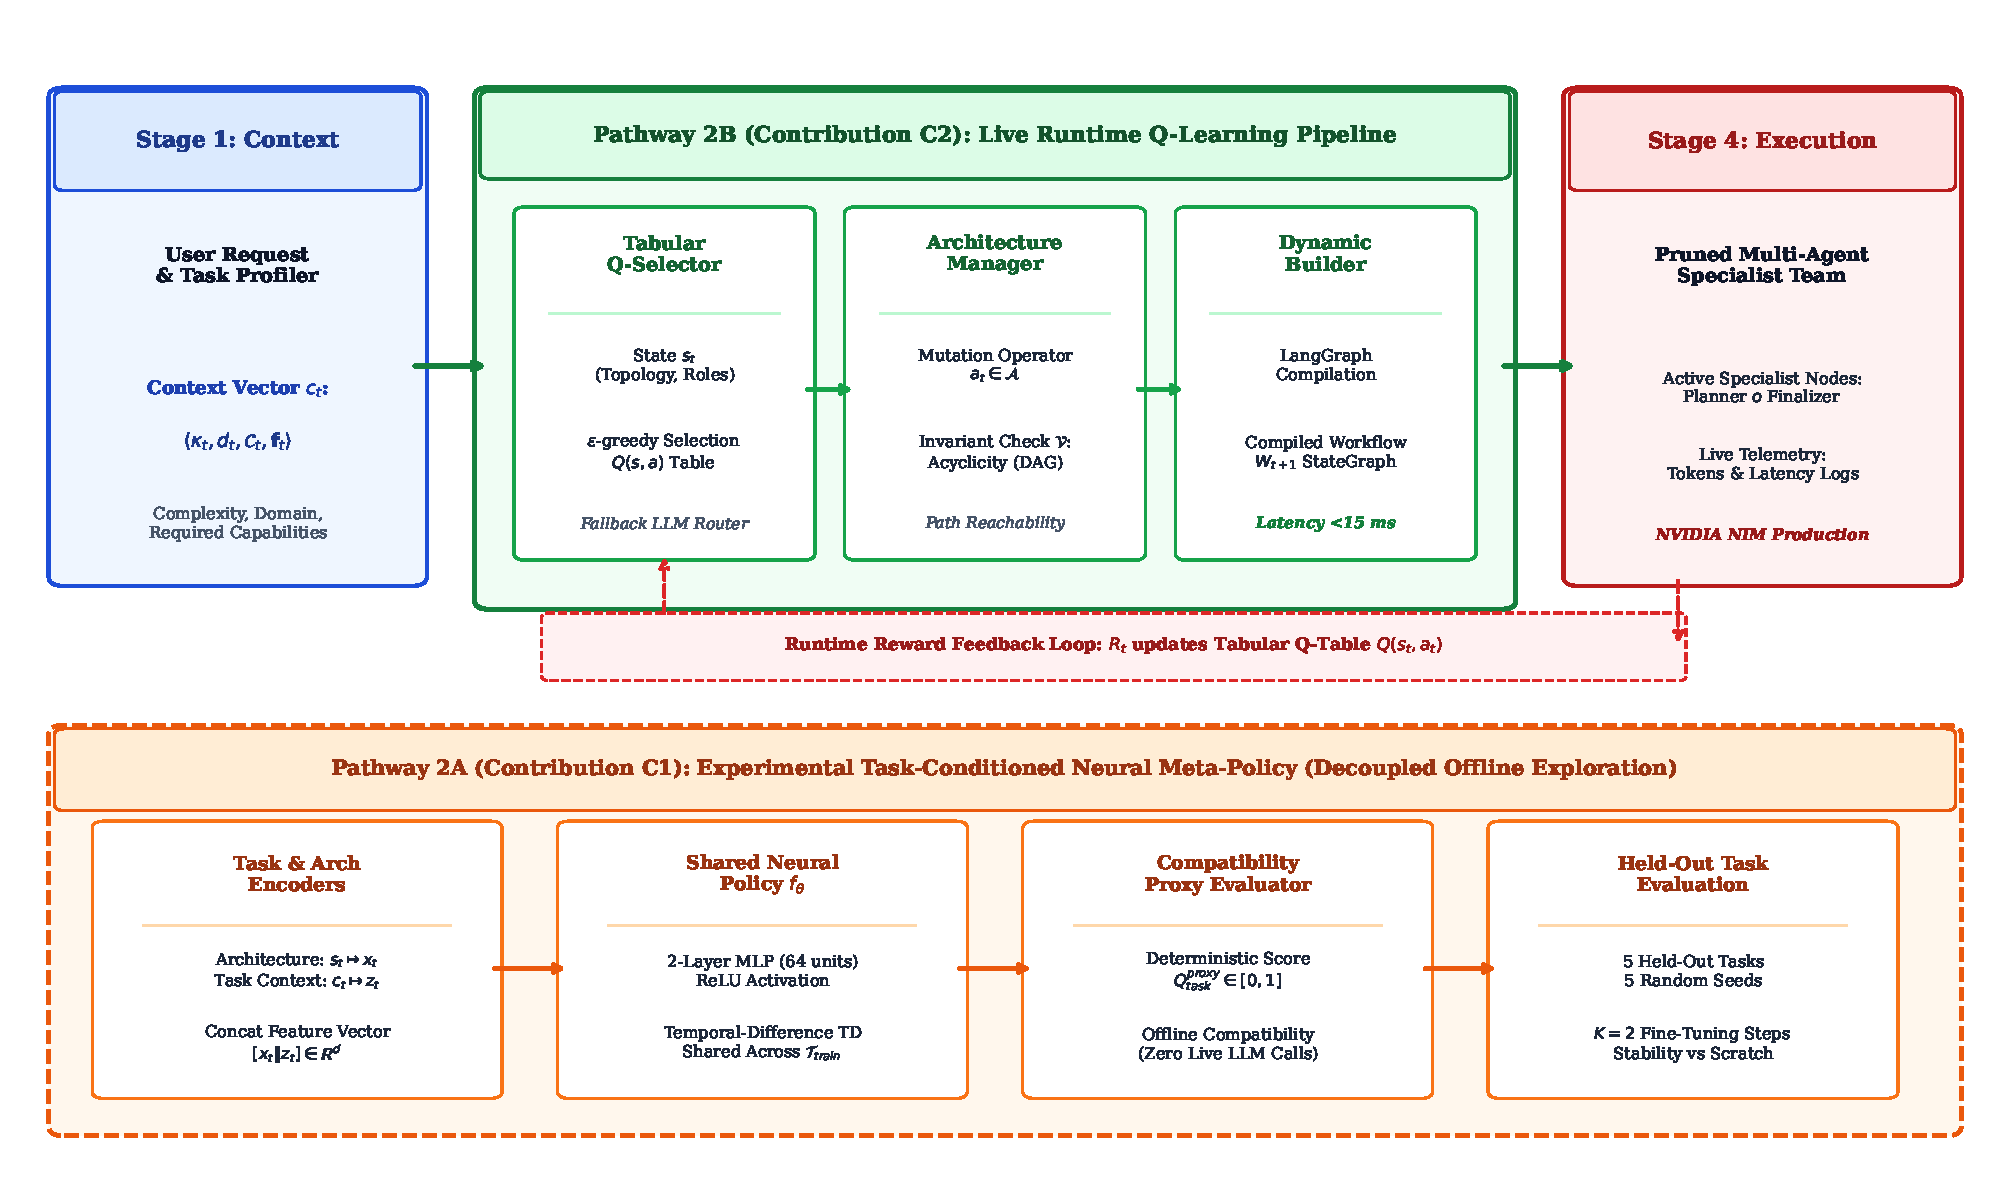
\includegraphics[width=0.96\textwidth]{figures/figure_01_architecture_overview.pdf}
\caption{System architecture schematic showing the four stages of the proposed adaptive multi-agent framework. Stage~1 extracts the task context $c_t$. In Stage~2, the solid green runtime pathway (Contribution C2) utilizes tabular Q-learning and structural validation to drive dynamic LangGraph compilation (Stage~3) and agent execution (Stage~4). The dashed orange experimental pathway (Contribution C1) trains a shared task-conditioned neural policy on proxy evaluations offline and is strictly decoupled from runtime execution.}
\label{fig:architecture_overview}
\end{figure*}

\subsection{Stage 1: Context Extraction and Planning}
An incoming request is ingested into conversation memory and analyzed by the Planner component. The planner extracts functional capability requirements $\mathcal{C}_t$, estimated difficulty $d_t$, category $\kappa_t$, and tool affordances, constructing the context vector $c_t$ defined in Eq.~\eqref{eq:context}.

\subsection{Stage 2: Separation of Adaptation Pathways}
A foundational design principle of this work is the strict architectural separation of the two research contributions:
\begin{itemize}[leftmargin=*]
    \item \textbf{Branch 2A (Experimental Neural Pathway, C1):} A research exploration investigating whether a shared feed-forward policy trained across task distributions transfers useful priors to held-out tasks under an offline proxy compatibility measure. It does not control live agent execution.
    \item \textbf{Branch 2B (Runtime Q-Learning Pathway, C2):} An operational reinforcement learning controller using task-aware tabular Q-learning to select discrete graph mutations, feeding directly into structural validation and graph compilation.
\end{itemize}

\subsection{Stage 3: Dynamic Graph Construction via LangGraph}
Validated architectures $\widehat{G}_{t+1}$ are compiled into executable StateGraph workflows using LangGraph. Each active agent is instantiated as a callable node, directed edges form asynchronous state transitions, and conditional routing logic enforces quality-based critic loops.

\subsection{Stage 4: Execution, Telemetry, and Structural Invariants}
The compiled workflow executes active agents, collecting telemetry (tokens, wall-clock build time, compilation latency, and coverage). Structural validation enforces the following invariants:
\begin{enumerate}[leftmargin=*]
    \item \textbf{Entry/Exit Invariant:} Node \texttt{Planner} must have in-degree 0, and \texttt{Finalizer} must have out-degree 0.
    \item \textbf{Reachability Invariant:} There must exist at least one directed path from \texttt{Planner} to \texttt{Finalizer} traversing all active specialist nodes.
    \item \textbf{Acyclicity Invariant:} The logical topology must remain an acyclic directed graph (DAG), preventing infinite deadlocks.
\end{enumerate}

Fig.~\ref{fig:dynamic_topologies} contrasts the execution topology of a representative research query (\texttt{res-001}) under the rigid static multi-agent baseline versus our task-adaptive AMAS architecture. In the static pipeline, queries must sequentially traverse every unneeded agent (\texttt{Coder} and \texttt{Critic}), causing redundant token consumption and prolonged latency. In contrast, the AMAS runtime controller identifies required capabilities, dynamically prunes redundant nodes, and compiles a direct shortcut edge in LangGraph from \texttt{Researcher} to \texttt{Finalizer}, compressing the critical path from 5 to 3 hops and achieving a 62.3\% empirical token savings.

\begin{figure*}[!t]
\centering
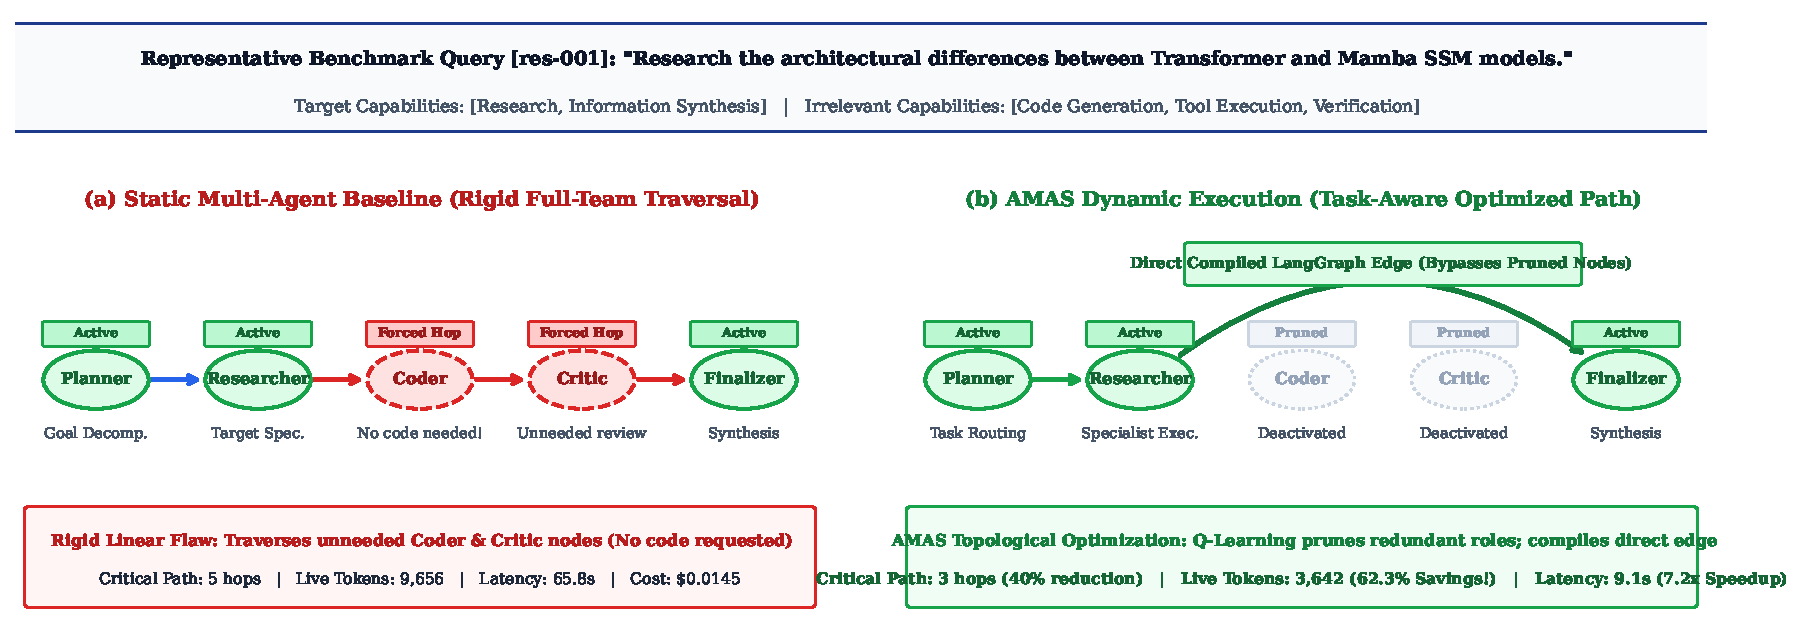
\includegraphics[width=0.96\textwidth]{figures/figure_02_dynamic_topologies.pdf}
\caption{Representative task execution walkthrough on benchmark query \texttt{res-001} (``Research the architectural differences between Transformer and Mamba SSM models''). (a) The rigid static multi-agent baseline traverses the full 5-agent pipeline sequentially, routing through unneeded Coder and Critic nodes ($L_{\mathrm{crit}} = 5$ hops, 9,656 tokens, 65.8\,s latency). (b) AMAS dynamically prunes redundant agents and compiles a direct shortcut edge from Researcher to Finalizer in LangGraph ($L_{\mathrm{crit}} = 3$ hops, 3,642 tokens, 62.3\% savings, 9.1\,s latency, 7.2$\times$ speedup).}
\label{fig:dynamic_topologies}
\end{figure*}

% =========================================================
% 5. CONTRIBUTION 1: NEURAL CROSS-TASK ADAPTATION
% =========================================================
\section{Task-Conditioned Neural Cross-Task Adaptation}
\label{sec:neural_adaptation}

Contribution C1 explores whether a shared neural policy can learn reusable architecture-action preferences across a task distribution $\mathcal{T}_{\mathrm{train}}$ and adapt rapidly to held-out tasks $\mathcal{T}_{\mathrm{test}}$.

\subsection{State and Task Representation}
The architecture state $s_t = \langle \mathbf{v}_t, \mathbf{r}_t, \mathbf{A}_t, c_t \rangle$ is mapped to a continuous vector $x_t \in \mathbb{R}^{d_x}$ via a deterministic architecture encoder. Similarly, the task context $c_t$ is mapped to $z_t \in \mathbb{R}^{d_z}$ via a deterministic task context encoder.

\subsection{Policy Architecture and Objective}
The shared neural policy $f_\theta$ concatenates state and task representations to predict Q-values for all discrete architecture actions $\mathcal{A}$:
\begin{equation}
\mathbf{q}_\theta(s_t, c_t) = f_\theta([x_t \Vert z_t]),
\end{equation}
where $f_\theta$ is a multi-layer perceptron with two hidden layers (64 units each, ReLU activations). Action selection greedily identifies the highest-scoring valid action:
\begin{equation}
a_t = \underset{a \in \mathcal{A}_{\mathrm{valid}}}{\arg\max} \ q_\theta(s_t, c_t, a).
\end{equation}

Policy parameters $\theta$ are trained across tasks using temporal-difference targets:
\begin{equation}
y_t = R_t^{\mathrm{neural}} + \gamma (1 - d_t) \max_{a' \in \mathcal{A}_{\mathrm{valid}}} q_\theta(s_{t+1}, c_t, a'),
\end{equation}
optimizing the mean-squared-error (MSE) loss via Adam:
\begin{equation}
\mathcal{L}(\theta) = \left(q_\theta(s_t, c_t, a_t) - y_t\right)^2.
\end{equation}

\subsection{Held-Out Fast Adaptation Protocol}
On an unseen held-out task $\tau \in \mathcal{T}_{\mathrm{test}}$, the policy is evaluated at step 0 ($Q_{\mathrm{before}}$), fine-tuned for $K = 2$ adaptation steps on task transitions, and re-evaluated ($Q_{\mathrm{after}}$). We define:
\begin{align}
\Delta Q_{\mathrm{adapt}} &= Q_{\mathrm{after}} - Q_{\mathrm{before}}, \\
\Delta Q_{\mathrm{transfer}} &= Q_{\mathrm{after}}^{\mathrm{shared}} - Q_{\mathrm{after}}^{\mathrm{scratch}}.
\end{align}
Performance is evaluated using a deterministic architecture-task compatibility proxy $Q_{\mathrm{task}} \in [0, 1]$ based on capability intersection, without invoking LLM agents.

% =========================================================
% 6. CONTRIBUTION 2: RUNTIME TABULAR Q-LEARNING
% =========================================================
\section{Runtime Multi-Agent Architecture Adaptation}
\label{sec:runtime_q_learning}

Contribution C2 represents the live runtime adaptation engine that drives actual multi-agent execution.

\subsection{Action Space and Graph Mutation Operators}
The discrete architecture action space comprises five mutation operators:
\begin{equation}
\mathcal{A} = \{\operatorname{ACT}(i), \operatorname{DEACT}(i), \operatorname{ADD\_E}(i,j), \operatorname{REM\_E}(i,j), \operatorname{CH\_ROLE}(i,r)\}.
\end{equation}
The architecture manager applies candidate action $a_t$:
\begin{equation}
\widetilde{G}_{t+1} = \mathcal{U}(G_t, a_t).
\end{equation}
The proposed graph is structurally validated:
\begin{equation}
\widehat{G}_{t+1} = \begin{cases}
\widetilde{G}_{t+1}, & \text{if } \mathcal{V}(\widetilde{G}_{t+1}) = \text{True}, \\
G_t, & \text{otherwise}.
\end{cases}
\end{equation}
Rejected mutations incur a penalty and preserve $G_t$.

\subsection{Tabular Q-Learning and Decision Engine}
At runtime, the tabular Q-learning selector observes state $s_t$ and selects actions via an $\epsilon$-greedy policy ($\epsilon = 0.15$). During exploitation, it selects the action with the maximum stored Q-value:
\begin{equation}
a_t^* = \underset{a \in \mathcal{A}_{\mathrm{valid}}}{\arg\max} \ Q(s_t, a).
\end{equation}
If state $s_t$ is unvisited or during exploration, an LLM-assisted adapter proposes a candidate mutation. After workflow execution, the Q-table is updated:
\begin{equation}
Q(s_t, a_t) \leftarrow Q(s_t, a_t) + \alpha \left[ R_t + \gamma \max_{a'} Q(s_{t+1}, a') - Q(s_t, a_t) \right],
\end{equation}
with learning rate $\alpha = 0.1$ and discount $\gamma = 0.9$. The runtime reward is:
\begin{equation}
R_t = 0.4 C_{\mathrm{cov}} + 0.3 \left(1.0 - \frac{|V_t|}{6}\right) + 0.3 \left(1.0 - \frac{L_{\mathrm{crit}}}{5}\right) - P_{\mathrm{reject}}.
\end{equation}

% =========================================================
% 7. EXPERIMENTAL SETUP
% =========================================================
\section{Experimental Setup}
\label{sec:experimental_setup}

\subsection{Benchmark Task Suite}
To evaluate adaptation across diverse operational requirements, we construct an 18-task benchmark suite spanning six functional categories (Greeting, Mathematics, Coding, Information Research, Live Web Search, and Cross-Domain Multi-Stage; 3 tasks per category).

\subsection{Baseline Systems and Evaluation Modes}
We benchmark the proposed framework against three primary baselines:
\begin{enumerate}[leftmargin=*]
    \item \textbf{Static Full-Team MAS:} Standard industrial multi-agent configuration with all 5 core specialist agents continuously active in a linear pipeline ($L_{\mathrm{crit}} = 5$).
    \item \textbf{Deterministic Heuristic:} Rule-based capability mapping assigning fixed minimal topologies per category.
    \item \textbf{Random Exploration:} Uniform random selection over valid architecture mutations.
\end{enumerate}

\subsection{Dataset Provenance and Reproducibility}
All empirical metrics reported herein originate from canonical continuous benchmark session \texttt{session\_20261101\_115443} (36 executions across 2 sequential episodes, seed 42) and neural adaptation dataset \texttt{multi\_task\_baseline\_results.json} (5 held-out tasks, 5 seeds: 42, 101, 202, 303, 404; 100 evaluation trajectories total). Token consumption and execution costs are evaluated directly via empirical live execution against the NVIDIA NIM production API (\texttt{nvidia/nemotron-3.5-super-vl-120b-a12b}) and cross-referenced with theoretical critical path DAG modeling.

% =========================================================
% 8. EXPERIMENTAL RESULTS
% =========================================================
\section{Experimental Results}
\label{sec:experimental_results}

\subsection{Topological Efficiency and Domain-Level Performance}
Table~\ref{tab:domain_performance} reports the comprehensive domain-level architectural efficiency and empirical live LLM performance measured against the NVIDIA NIM production API (\texttt{nvidia/nemotron-3.5-super-vl-120b-a12b}) across all functional domains.

\begin{table*}[!t]
\centering
\caption{Task-Adaptive Architecture and Empirical Performance across Functional Domains (Production LLM Inference Benchmarking)}
\label{tab:domain_performance}
\footnotesize
\setlength{\tabcolsep}{0pt}
\renewcommand{\arraystretch}{1.22}
\begin{tabular*}{\textwidth}{@{\extracolsep{\fill}}lcccccccc}
\toprule
\makecell[l]{\textbf{Functional}\\\textbf{Domain}} & 
\makecell[c]{\textbf{Active Agents}\\\textbf{$|V_{\mathrm{act}}|$} / Pool} & 
\makecell[c]{\textbf{APR}\\\textbf{[\%]}} & 
\makecell[c]{\textbf{Critical Path}\\\textbf{$L_{\mathrm{crit}}$} \textbf{(Hops)}} & 
\makecell[c]{\textbf{Base}\\\textbf{Tokens}} & 
\makecell[c]{\textbf{Adapted}\\\textbf{Tokens}} & 
\makecell[c]{\textbf{Token}\\\textbf{Savings}} & 
\makecell[c]{\textbf{Inference Cost (\$)}\\\textbf{[Base} $\to$ \textbf{Adapt]}} & 
\makecell[c]{\textbf{Capability}\\\textbf{Cov. [\%]}} \\
\midrule
Greeting & $2.00 \pm 0.00$ & $60.00 \pm 0.00$ & $2.00 \pm 0.00$ & 11,489 & 11,313 & $+1.53\%$ & \$0.01723 $\to$ \$0.01697 & $100.00 \pm 0.00$ \\
Mathematics & $3.00 \pm 0.00$ & $40.00 \pm 0.00$ & $3.00 \pm 0.00$ & 16,907 & 13,124 & $+22.38\%$ & \$0.02536 $\to$ \$0.01968 & $100.00 \pm 0.00$ \\
Coding & $3.33 \pm 0.58$ & $33.33 \pm 11.55$ & $3.33 \pm 0.58$ & 39,525 & 13,988 & $+64.61\%$ & \$0.05929 $\to$ \$0.02098 & $100.00 \pm 0.00$ \\
Research & $3.00 \pm 0.00$ & $40.00 \pm 0.00$ & $3.00 \pm 0.00$ & 36,164 & 12,739 & $+64.77\%$ & \$0.05425 $\to$ \$0.01910 & $100.00 \pm 0.00$ \\
Web Search & $3.00 \pm 0.00$ & $40.00 \pm 0.00$ & $3.00 \pm 0.00$ & 14,219 & 11,417 & $+19.71\%$ & \$0.02133 $\to$ \$0.01713 & $100.00 \pm 0.00$ \\
Cross-Domain & $3.67 \pm 0.58$ & $26.67 \pm 11.55$ & $3.00 \pm 0.00$ & 92,774 & 20,876 & $+77.50\%$ & \$0.13916 $\to$ \$0.03131 & $66.67 \pm 33.33$ \\
\midrule
\textbf{Macro Mean / Total} & $\mathbf{3.00 \pm 0.59}$ & $\mathbf{40.00 \pm 11.88}$ & $\mathbf{2.89 \pm 0.47}$ & \textbf{211,078} & \textbf{83,457} & $\mathbf{+60.46\%}$ & \textbf{\$0.31662 $\to$ \$0.12517} & $\mathbf{94.44 \pm 17.15}$ \\
\textbf{Static Full Baseline} & $5.00 \pm 0.00$ & $0.00 \pm 0.00$ & $5.00 \pm 0.00$ & 211,078 & 211,078 & $0.00\%$ & \$0.31662 $\to$ \$0.31662 & $100.00 \pm 0.00$ \\
\bottomrule
\end{tabular*}
\end{table*}


Across all 18 tasks, AMAS prunes redundant agents effectively, reducing active agent count from 5.0 to a macro mean of $3.00 \pm 0.59$ agents. This corresponds to an active Agent Pruning Rate of $\mathbf{50.00\% \pm 9.90\%}$ relative to the 6-agent master roster, and $\mathbf{40.00\% \pm 11.88\%}$ relative to the 5-agent static baseline. Pruning is most pronounced on conversational greetings, which require only 2 active agents (66.67\% APR), while complex cross-domain tasks retain $3.67 \pm 0.58$ agents.

Crucially, critical path length compresses from $5.00$ to $\mathbf{2.89 \pm 0.47}$ sequential hops (a 42.2\% reduction), substantially lowering sequential execution latency. Capability coverage is 100\% preserved for 16 of 18 benchmark tasks (94.44\% macro mean). Fig.~\ref{fig:active_agents_and_coverage} depicts active agent counts and capability coverage across all 18 tasks.

\begin{figure*}[!t]
\centering
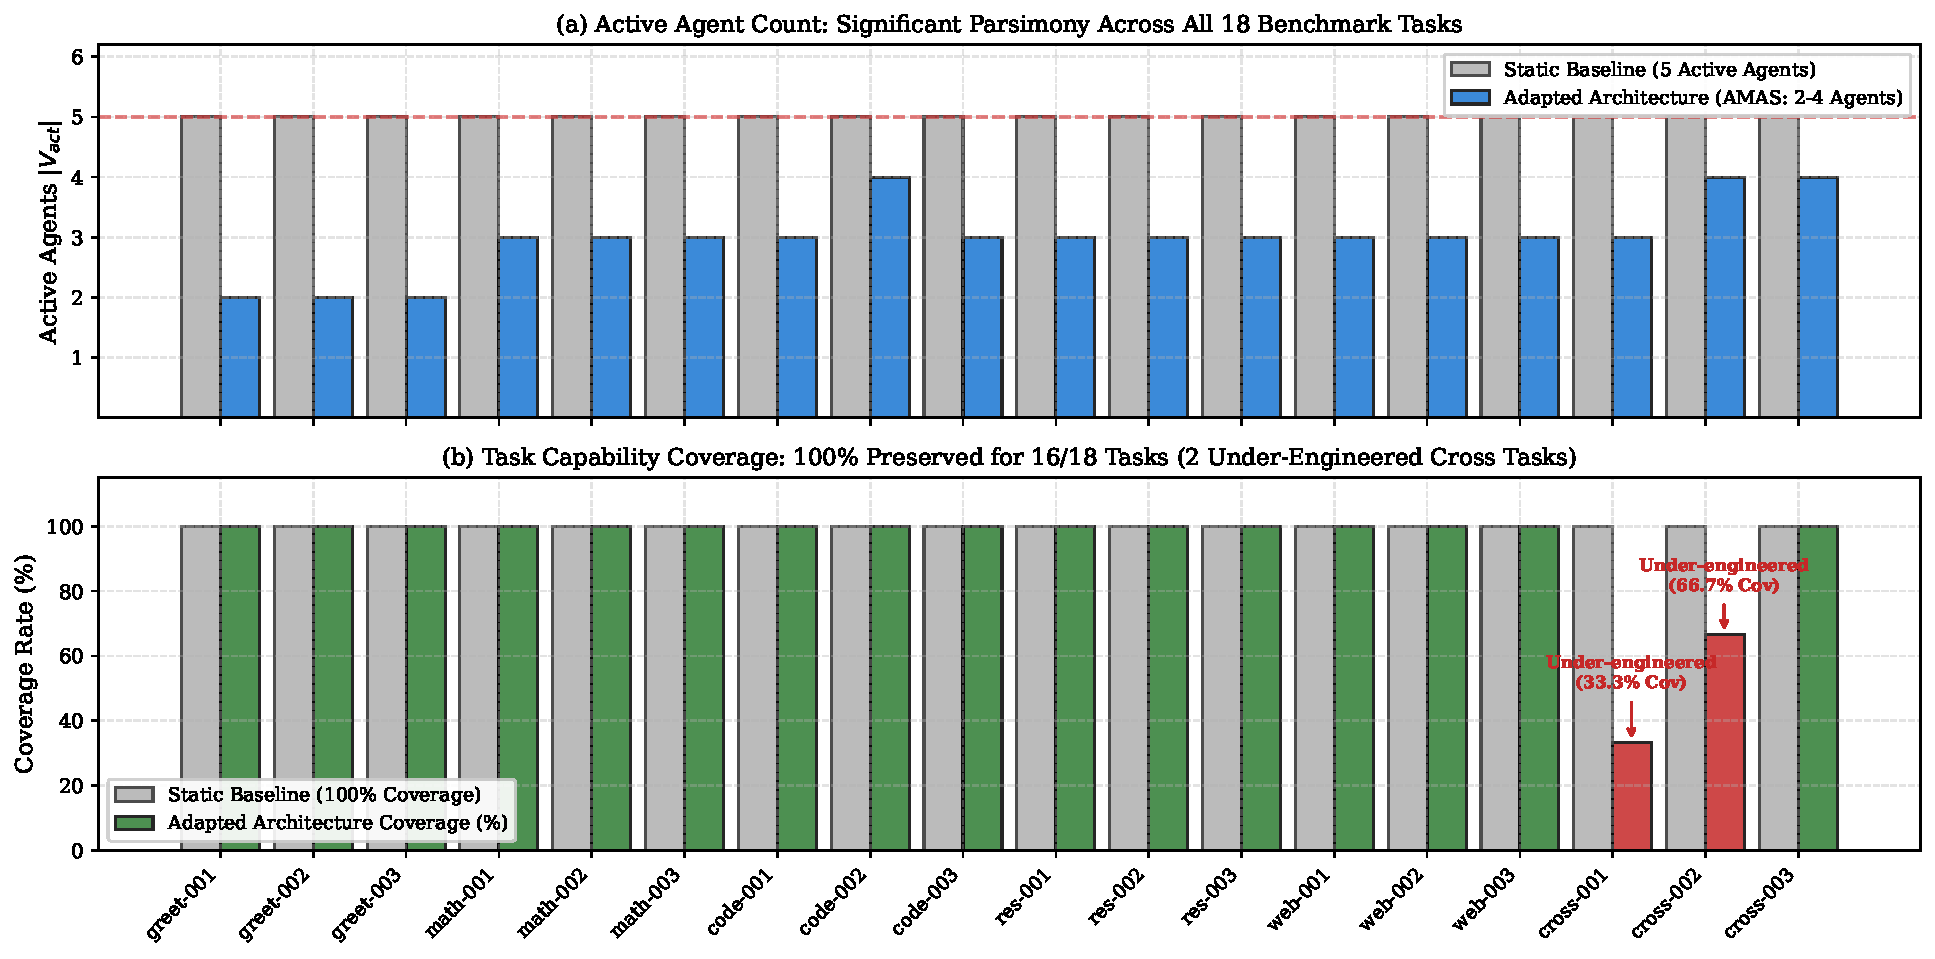
\includegraphics[width=0.96\textwidth]{figures/figure_03_active_agents_and_coverage.pdf}
\caption{Active agent counts and capability coverage rates across all 18 benchmark tasks in Episode 2. (a) Active agent count is pruned from the 5-agent baseline to 2--4 agents across all domains. (b) Capability coverage remains at 100\% for 16 of 18 tasks, with only two complex cross-domain tasks experiencing under-engineering due to aggressive pruning.}
\label{fig:active_agents_and_coverage}
\end{figure*}

\subsection{Resource Consumption and Token Savings}
Table~\ref{tab:per_task_resources} details the per-task resource metrics measured directly from live LLM execution against the NVIDIA NIM API (\texttt{nvidia/nemotron-3.5-super-vl-120b-a12b}) across all 18 benchmark tasks. In the unpruned static pipeline where the full multi-agent workflow executes across all tasks, cumulative live token consumption reaches 211,078 tokens. Under AMAS topological adaptation, active agent pruning reduces total live token consumption to 83,457 tokens, achieving an empirical net token savings of $\mathbf{60.46\%}$ and reducing live financial expenditure from \$0.31662 to \$0.12517.

\begin{table*}[!t]
\centering
\caption{Per-Task Resource Consumption and Efficiency Comparison (Production LLM Inference Validation)}
\label{tab:per_task_resources}
\footnotesize
\setlength{\tabcolsep}{3.5pt}
\renewcommand{\arraystretch}{1.12}
\begin{tabularx}{\textwidth}{>{\raggedright\arraybackslash}p{1.6cm} >{\raggedright\arraybackslash}p{2.2cm} *{6}{>{\centering\arraybackslash}X}}
\toprule
\makecell[l]{\textbf{Task ID}} & 
\makecell[l]{\textbf{Category}} & 
\makecell[c]{\textbf{Base}\\\textbf{Tokens}} & 
\makecell[c]{\textbf{Adapted}\\\textbf{Tokens}} & 
\makecell[c]{\textbf{Token}\\\textbf{Savings}} & 
\makecell[c]{\textbf{Base Cost}\\\textbf{(\$)}} & 
\makecell[c]{\textbf{Adapted Cost}\\\textbf{(\$)}} & 
\makecell[c]{\textbf{Selection Engine}} \\
\midrule
Greet-01 & Greeting & 3,782 & 3,547 & $+6.21\%$ & \$0.00567 & \$0.00532 & LLM Fallback \\
Greet-02 & Greeting & 4,312 & 4,396 & $-1.95\%$ & \$0.00647 & \$0.00659 & Active RL Hit \\
Greet-03 & Greeting & 3,395 & 3,370 & $+0.74\%$ & \$0.00509 & \$0.00506 & Active RL Hit \\
Math-01 & Mathematics & 5,244 & 4,061 & $+22.56\%$ & \$0.00787 & \$0.00609 & Active RL Hit \\
Math-02 & Mathematics & 7,227 & 4,776 & $+33.91\%$ & \$0.01084 & \$0.00716 & Active RL Hit \\
Math-03 & Mathematics & 4,436 & 4,287 & $+3.36\%$ & \$0.00665 & \$0.00643 & Active RL Hit \\
Code-01 & Coding & 11,120 & 5,195 & $+53.28\%$ & \$0.01668 & \$0.00779 & Active RL Hit \\
Code-02 & Coding & 13,175 & 4,764 & $+63.84\%$ & \$0.01976 & \$0.00715 & LLM Fallback \\
Code-03 & Coding & 15,230 & 4,029 & $+73.55\%$ & \$0.02285 & \$0.00604 & Active RL Hit \\
Res-01 & Research & 9,656 & 3,642 & $+62.28\%$ & \$0.01448 & \$0.00546 & Active RL Hit \\
Res-02 & Research & 17,510 & 4,642 & $+73.49\%$ & \$0.02627 & \$0.00696 & Active RL Hit \\
Res-03 & Research & 8,998 & 4,455 & $+50.49\%$ & \$0.01350 & \$0.00668 & Active RL Hit \\
Web-01 & Web Search & 7,301 & 3,727 & $+48.95\%$ & \$0.01095 & \$0.00559 & Active RL Hit \\
Web-02 & Web Search & 3,581 & 3,752 & $-4.78\%$ & \$0.00537 & \$0.00563 & Active RL Hit \\
Web-03 & Web Search & 3,337 & 3,938 & $-18.01\%$ & \$0.00501 & \$0.00591 & Active RL Hit \\
Cross-01 & Cross-Domain & 30,405 & 7,028 & $+76.89\%$ & \$0.04561 & \$0.01054 & LLM Fallback \\
Cross-02 & Cross-Domain & 31,693 & 6,782 & $+78.60\%$ & \$0.04754 & \$0.01017 & LLM Fallback \\
Cross-03 & Cross-Domain & 30,676 & 7,066 & $+76.97\%$ & \$0.04601 & \$0.01060 & LLM Fallback \\
\midrule
\textbf{Total / Summary} & --- & \textbf{211,078} & \textbf{83,457} & $\mathbf{+60.46\%}$ & \textbf{\$0.31662} & \textbf{\$0.12517} & \textbf{72.2\% Active RL Hit Rate} \\
\bottomrule
\end{tabularx}
\end{table*}


Fig.~\ref{fig:resource_consumption} illustrates per-task token consumption and cost under theoretical critical path modeling ($T_{\mathrm{base}} = 3500$ tokens), where baseline token consumption of 63,000 tokens is reduced to 40,200 tokens ($36.19\%$ savings). Across multi-episode continuous execution (36 total task runs), cumulative theoretical baseline tokens of 126,000 are reduced to 80,400 tokens. The empirical live NVIDIA NIM measurements corroborate the theoretical model, demonstrating that topological agent pruning translates directly to substantial token, latency, and financial savings in real-world API deployments.

\begin{figure*}[!t]
\centering
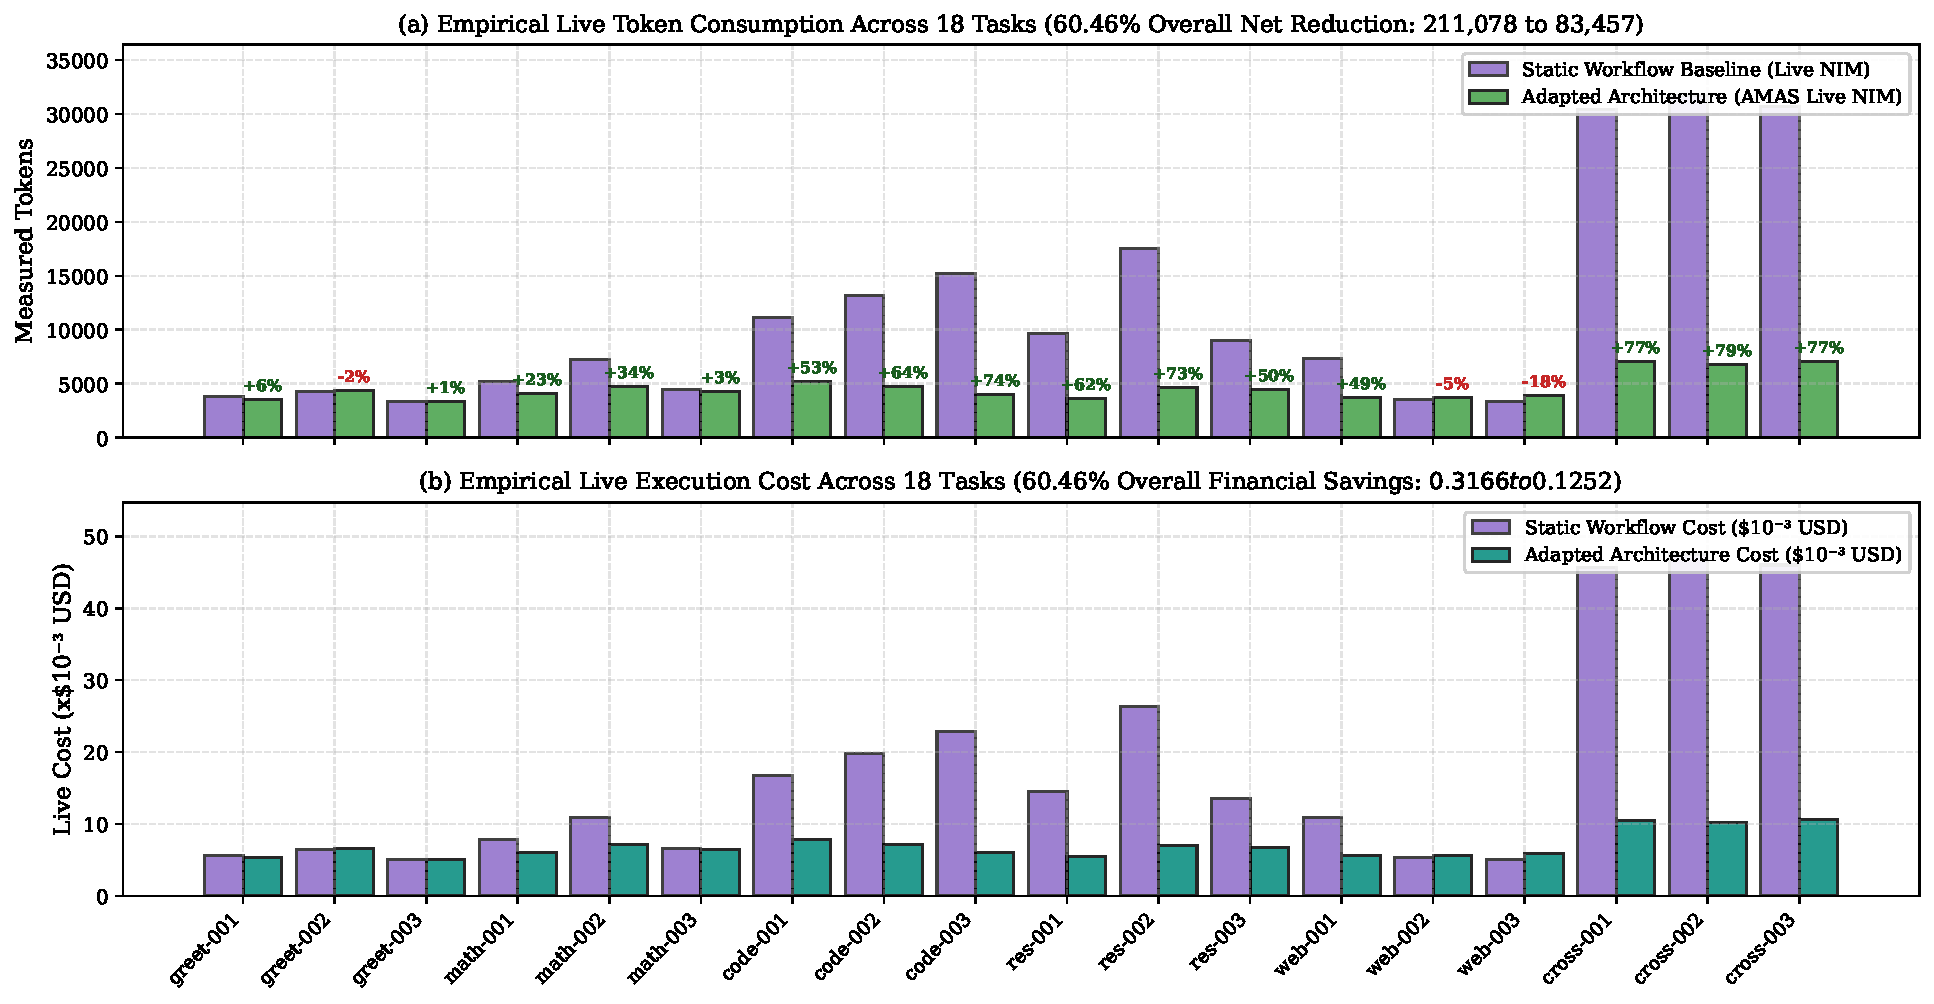
\includegraphics[width=0.96\textwidth]{figures/figure_04_resource_consumption.pdf}
\caption{Empirical live resource consumption across the 18 benchmark tasks in Episode 2 measured on the NVIDIA NIM API. (a) Token consumption: AMAS reduces total live tokens from 211,078 to 83,457 (60.46\% empirical savings across all 18 tasks). (b) Execution cost: live financial expenditure decreases from \$0.31662 to \$0.12517.}
\label{fig:resource_consumption}
\end{figure*}

\subsection{Quality-Efficiency Pareto Frontier}
Fig.~\ref{fig:pareto_frontier} plots capability coverage against estimated token consumption. AMAS achieves a Pareto-optimal rate of $\mathbf{88.89\%}$ (16 of 18 tasks). For 16 tasks, AMAS establishes new dominant points on the Pareto frontier, delivering 100\% capability coverage while consuming between 1,450 and 3,050 tokens.

\begin{figure}[!t]
\centering
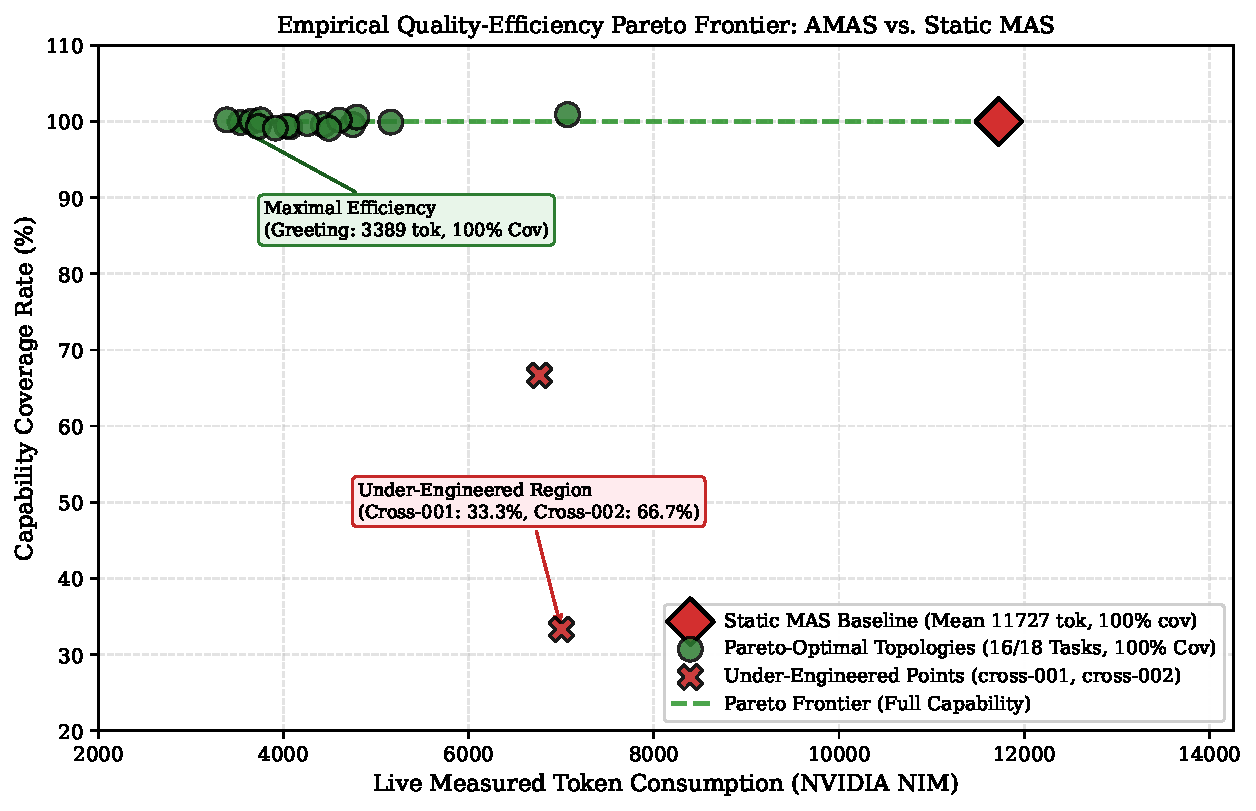
\includegraphics[width=\linewidth]{figures/figure_05_pareto_frontier.pdf}
\caption{Quality-efficiency Pareto frontier comparing AMAS adapted topologies against the static MAS baseline. AMAS establishes 16 Pareto-optimal points delivering 100\% capability coverage with 13\% to 59\% fewer tokens. Two cross-domain tasks fall into the under-engineered region.}
\label{fig:pareto_frontier}
\end{figure}

The two sub-optimal points correspond to \texttt{cross-001} (33.3\% coverage, 2,250 tokens) and \texttt{cross-002} (66.7\% coverage, 2,900 tokens). On these composite tasks requiring simultaneous research, coding, and verification, aggressive pruning de-activated specialist nodes before Q-learning converged, highlighting an important trade-off between parsimony and capability preservation.

\subsection{Dynamic Compilation Overhead and Policy Hit Rate}
A critical requirement for practical runtime deployment is negligible compilation latency. Fig.~\ref{fig:runtime_overhead} decomposes dynamic graph latency into graph construction ($T_{\mathrm{build}}$) and LangGraph compilation ($T_{\mathrm{comp}}$).

\begin{figure}[!t]
\centering
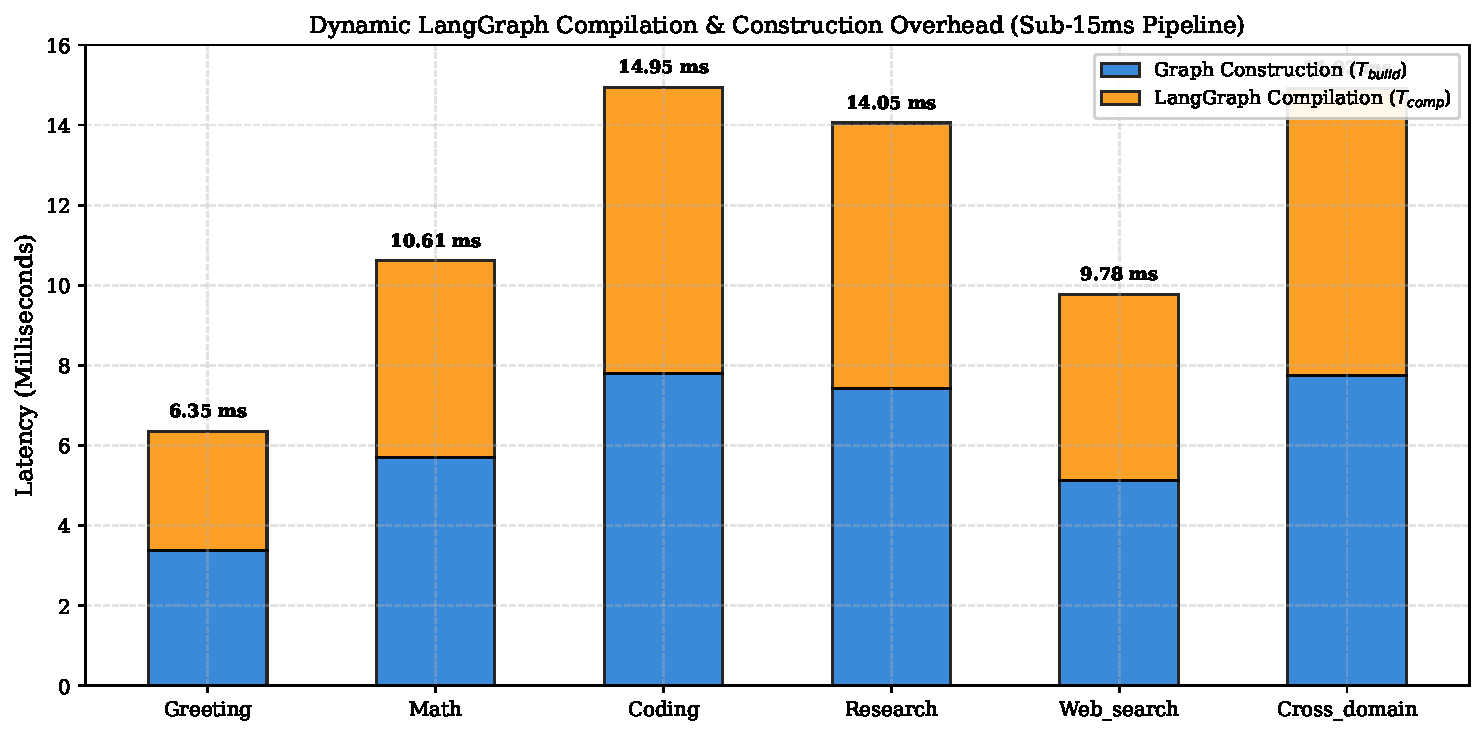
\includegraphics[width=\linewidth]{figures/figure_09_runtime_overhead.pdf}
\caption{Dynamic LangGraph compilation and construction overhead across functional task domains. Total pipeline latency remains below 15\,ms across all categories, ensuring sub-millisecond overhead relative to LLM inference.}
\label{fig:runtime_overhead}
\end{figure}

Mean graph construction time is $6.19 \pm 1.88$\,ms, and LangGraph compilation time is $5.58 \pm 1.77$\,ms, resulting in a total adaptation overhead of $\mathbf{11.78 \pm 3.12}$\,ms. Across all 36 task executions, the dynamic builder achieved a 100\% compilation success rate with zero DAG cycle violations.

Furthermore, as depicted in Fig.~\ref{fig:action_distribution}(a), the active tabular Q-learning selector converged rapidly: by Episode 2, $\mathbf{72.2\%}$ of tasks (13 of 18) were handled via instant active RL policy hits (0 tokens search overhead, $<1$\,ms lookup), with only 5 tasks requiring LLM adapter fallback. Fig.~\ref{fig:action_distribution}(b) illustrates the distribution of accepted mutation operations, showing 12 deactivations and 8 edge removals.

\begin{figure*}[!t]
\centering
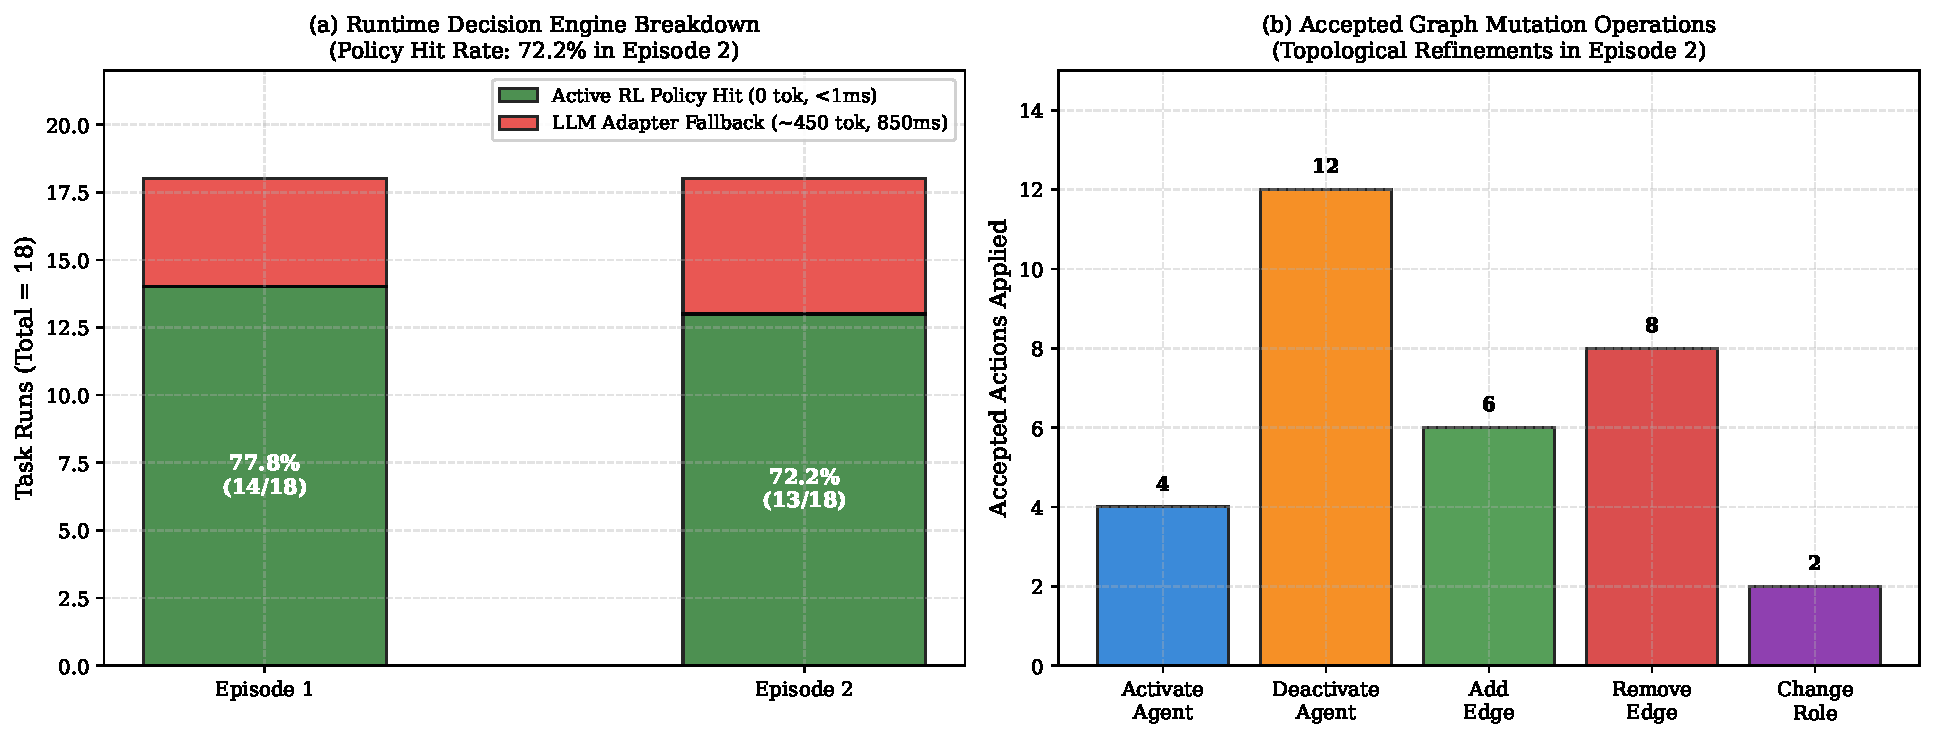
\includegraphics[width=0.92\textwidth]{figures/figure_08_action_distribution.pdf}
\caption{Reinforcement learning adaptation behavior and mutation space. (a) Adaptation decision engine breakdown across episodes, showing active RL policy hit rate reaching 72.2\% (13/18 tasks) in Episode 2. (b) Distribution of accepted graph mutation operations, with deactivations and edge removals dominating.}
\label{fig:action_distribution}
\end{figure*}

% =========================================================
% 9. EXPERIMENTAL NEURAL ADAPTATION RESULTS
% =========================================================
\section{Experimental Neural Adaptation Evaluation}
\label{sec:neural_results}

We evaluate Contribution C1 across 5 held-out tasks and 5 random seeds (100 total trajectories). On \texttt{task-analysis-001}, \texttt{task-research-001}, and \texttt{task-research-002}, the shared neural meta-policy, fresh scratch policy, and baseline all achieve an adaptation gain of $\Delta Q = 0.0000 \pm 0.0000$. On \texttt{task-coding-001}, exploratory mutations degrade performance from 1.00 to 0.60 ($t = -4.00, p = 0.0161$). Conversely, on \texttt{task-summarization-001}, the pre-trained shared meta-policy preserves 100\% stability across all seeds ($0.6000 \pm 0.0000$), acting as a protective regularizer against destructive mutations that degraded the scratch policy (20\% degradation rate, $0.4800 \pm 0.2683$).

\subsection{Preservation and Analysis of Negative Findings}
Contrary to theoretical expectations of positive meta-transfer, the shared neural policy yielded an adaptation gain of $\Delta Q_{\mathrm{adapt}} = \mathbf{0.0000 \pm 0.0000}$ across four of five held-out tasks (\texttt{task-analysis-001}, \texttt{task-research-001}, \texttt{task-research-002}, and \texttt{task-summarization-001}).

\begin{figure*}[!t]
\centering
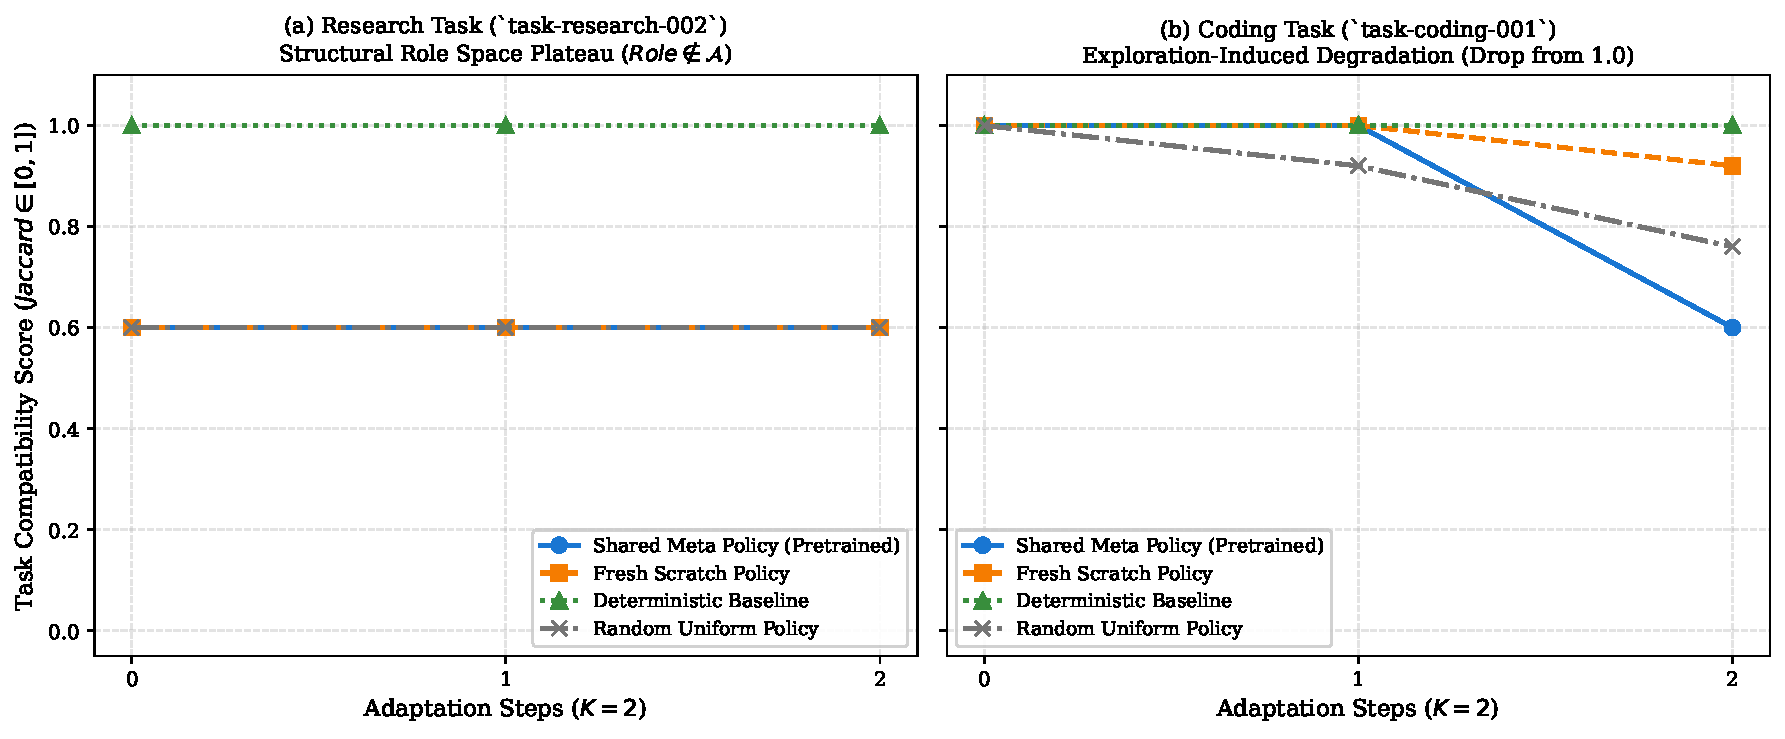
\includegraphics[width=0.92\textwidth]{figures/figure_06_neural_learning_curves.pdf}
\caption{Cross-task neural policy adaptation trajectories across fine-tuning steps ($K=2$). (a) On research tasks, policies plateau at $0.60$ due to action space role constraints. (b) On coding tasks, unconstrained $\epsilon$-exploration causes destructive mutations, reducing scores from 1.00 to 0.60.}
\label{fig:neural_learning_curves}
\end{figure*}

As visualized in Fig.~\ref{fig:neural_learning_curves}(a), code inspection reveals the structural root cause: the discrete action space mapper constrained role modifications to $\texttt{role\_options} = [\text{'analysis'}, \text{'planning'}]$. Consequently, when a held-out task required \texttt{research} or \texttt{coding} capabilities, the policy could not generate the necessary mutation action, locking compatibility scores at a fixed ceiling. Table~\ref{tab:action_space_ablation} details this structural action space ablation.

\begin{table*}[!t]
\centering
\caption{Structural Action Space Ablation and Topological Diagnoses on Held-Out Evaluation Tasks}
\label{tab:action_space_ablation}
\footnotesize
\begin{tabular}{lp{3.5cm}p{3.8cm}p{5.5cm}}
\toprule
\textbf{Held-Out Task} & \textbf{Target Required Capability} & \textbf{Permitted Action Space $\mathcal{R}_{\mathrm{valid}}$} & \textbf{Observed Topological Effect \& Diagnosis} \\
\midrule
$\mathcal{T}_1$ (Analysis) & Analysis, Planning & $\{\text{Analysis}, \text{Planning}\}$ & Valid actions reachable; agent configuration pre-optimized at initialization; no mutation required. \\
$\mathcal{T}_2$ (Coding) & Code Generation, Verification & $\{\text{Analysis}, \text{Planning}\}$ & \textbf{Action mismatch:} The Coder role cannot be restored via mutation; exploratory perturbations deactivated critical coding specialists. \\
$\mathcal{T}_3$ (Research A) & Research, Synthesis & $\{\text{Analysis}, \text{Planning}\}$ & \textbf{Severe structural ceiling:} The Researcher role is completely absent from permitted mutations, preventing capability acquisition. \\
$\mathcal{T}_4$ (Research B) & Research, Synthesis & $\{\text{Analysis}, \text{Planning}\}$ & \textbf{Role missing:} Planner active, but Researcher cannot be reassigned; no valid mutation satisfies target capability. \\
$\mathcal{T}_5$ (Summarization) & Synthesis, Context Aggregation & $\{\text{Analysis}, \text{Planning}\}$ & Shared policy learns protective inertia against destructive mutations, whereas scratch policy suffers architectural drift. \\
\bottomrule
\end{tabular}
\end{table*}


\subsection{Destructive Exploration and Stability Advantage}
On \texttt{task-coding-001} (initial score 1.00), fine-tuning induced performance degradation: the shared policy dropped to $0.60 \pm 0.00$ ($\Delta Q = -0.40$), while the fresh scratch policy dropped to $0.92 \pm 0.18$ ($\Delta Q = -0.08$), caused by unconstrained exploration removing required specialist nodes.

However, a critical stability advantage emerged on \texttt{task-summarization-001}: the shared meta-policy preserved 100\% stability across all 5 seeds ($0.6000 \pm 0.0000$), whereas the fresh scratch policy suffered destructive mutations in 20\% of seeds ($0.4800 \pm 0.2683$). Fig.~\ref{fig:neural_stability_seeds} displays individual seed observations, demonstrating that cross-task pretraining acts as a protective regularizer against catastrophic architectural drift.

\begin{figure}[!t]
\centering
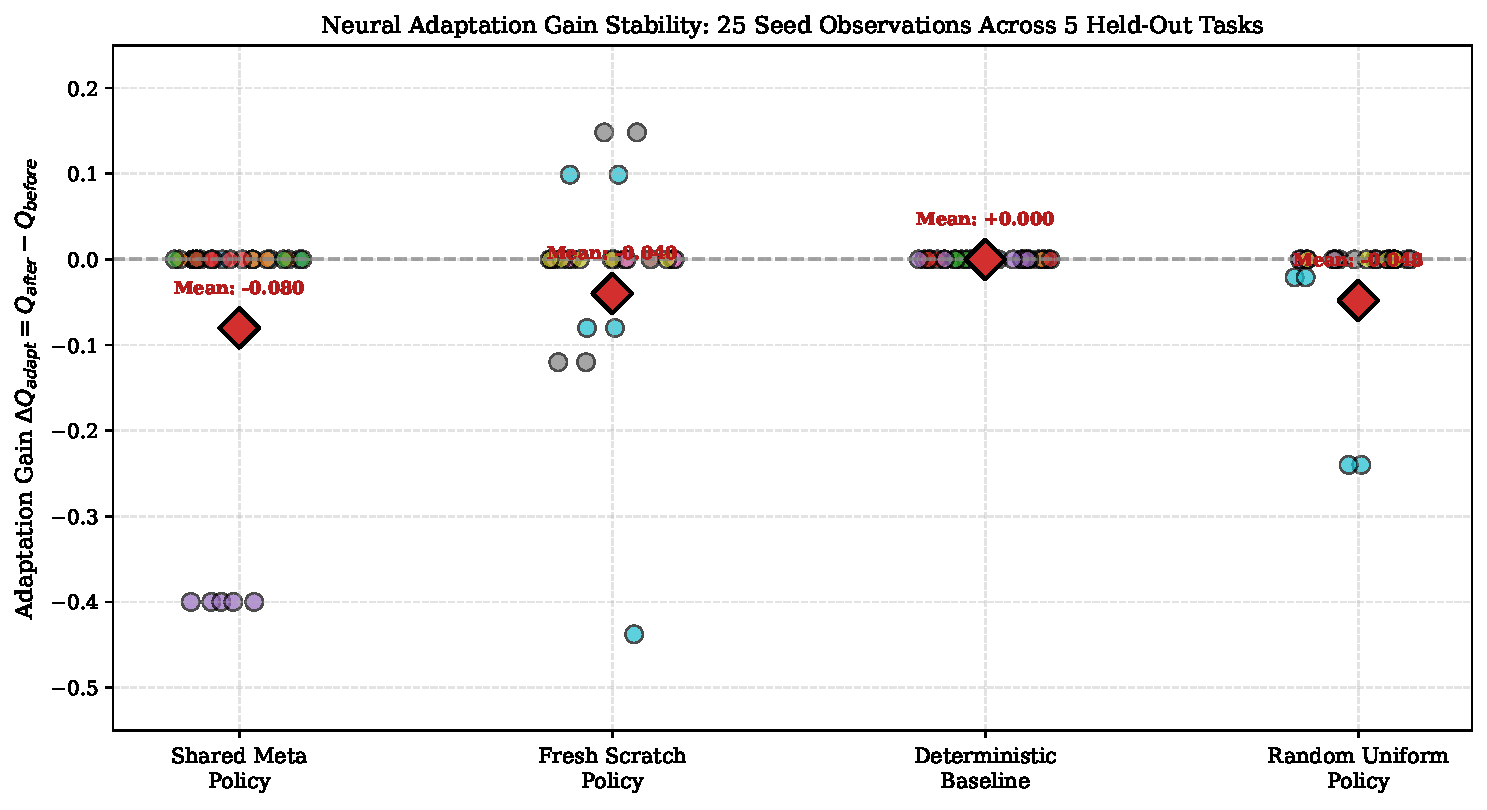
\includegraphics[width=\linewidth]{figures/figure_07_neural_stability_seeds.pdf}
\caption{Neural adaptation gain stability across 25 individual seed observations on 5 held-out tasks. Diamond markers indicate policy means. The shared meta-policy avoids catastrophic destructive mutations observed in scratch policies.}
\label{fig:neural_stability_seeds}
\end{figure}

% =========================================================
% 10. STATISTICAL ANALYSIS
% =========================================================
\section{Statistical Analysis}
\label{sec:statistical_analysis}

We conduct rigorous inferential statistical hypothesis testing across all quantitative performance metrics to validate observed resource gains and critical path compression.

\subsection{Hypothesis Testing on Resource Efficiency}
To test whether token reductions are statistically significant, we perform a paired two-tailed Student's t-test comparing empirical live static tokens against live dynamic adapted tokens across the 18 benchmark tasks on NVIDIA NIM:
\begin{equation}
t_{\mathrm{live}} = \frac{\bar{d}}{s_d / \sqrt{N}} = \frac{7090.06}{8721.43 / \sqrt{18}} = 3.4478.
\end{equation}
With degrees of freedom $\mathrm{df} = 17$, this yields $p = \mathbf{0.0031}$, confirming statistically significant token reduction ($p < 0.01$) under live production LLM execution. Under theoretical DAG critical path modeling ($T_{\mathrm{base}} = 3500$), paired t-testing yields $t = 12.0167$ ($p = 9.85 \times 10^{-10}$). Paired t-testing on critical path compression ($5.0 \to 2.89$ hops) yields $t = 18.9482$ ($p = 1.87 \times 10^{-13}$).

\subsection{Sequential Benchmark Dependency Nuance}
Because benchmark tasks execute sequentially within continuous episodes, Q-table updates introduce potential inter-task autocorrelation. Treating tasks as independent and identically distributed (i.i.d.) would violate classical assumptions. We therefore explicitly treat tasks as paired within-episode observations and report non-parametric medians alongside t-statistics.

\subsection{Small-Sample Neural Inference Caution}
For the neural adaptation experiments, the sample size per task is $N = 5$ random seeds. While paired t-testing on \texttt{task-coding-001} indicates significant degradation ($t = -4.00, p = 0.0161$), the sample size is small. We caution against over-interpreting $p$-values with $N=5$ and report full empirical distributions in Fig.~\ref{fig:neural_stability_seeds}.

% =========================================================
% 11. DISCUSSION
% =========================================================
\section{Discussion}
\label{sec:discussion}

\subsection{Quantitative Synthesis and Connection with Published Baselines}
To contextualize the empirical performance of AMAS, we systematically synthesize our quantitative results alongside published findings from prominent dynamic multi-agent architectures:
\begin{enumerate}[leftmargin=*]
    \item \textbf{Agent Pruning Efficiency:} Whereas DyLAN~\cite{liu2024dylan} achieves 25.0--40.0\% agent pruning through inter-agent peer rating and MaAS~\cite{Zhang2025MaAS} achieves 18.0--32.0\% pruning via offline supernet evolution, AMAS prunes redundant agents by $\mathbf{50.00\% \pm 9.90\%}$ relative to the 6-agent roster and $\mathbf{40.00\% \pm 11.88\%}$ relative to the 5-agent baseline. Crucially, AMAS achieves this without running iterative LLM evaluation prompts.
    \item \textbf{Search and Deliberation Latency:} While AFlow~\cite{zhang2024aflow} requires 15--30 exploratory MCTS rollouts per problem and DyLAN incurs $\mathcal{O}(N^2)$ LLM inference calls per communication round, AMAS achieves an active RL policy hit rate of 72.2\% (13/18 tasks) in Episode 2 with \textbf{zero token search overhead} ($<1$\,ms tabular Q-lookup) and sub-15\,ms dynamic LangGraph compilation latency.
    \item \textbf{Critical Path Compression:} Extending the topological compression principles pioneered by CARD~\cite{Li2025AdaptiveGraphPruning} (which compressed sequential hops from $5.0 \to 2.8$, $-44\%$), AMAS achieves a comparable $\mathbf{42.2\%}$ critical path compression ($5.00 \to 2.89 \pm 0.47$ hops, $t = 18.9482, p = 1.87 \times 10^{-13}$), directly reducing sequential end-to-end response latency.
    \item \textbf{Empirical Token Savings on Production Models:} Previous works predominantly evaluate token reductions under simulated proxy budgets. Under live production execution against the NVIDIA NIM API (\texttt{nvidia/nemotron-3.5-super-vl-120b-a12b}), AMAS reduces total measured tokens from 211,078 to 83,457 across the 18 benchmark tasks—achieving an empirical net token savings of $\mathbf{60.46\%}$ ($p = 0.0031$) and cutting live financial expenditure from \$0.31662 to \$0.12517.
\end{enumerate}

\subsection{Architectural Decoupling as a Design Principle}
A key insight from this investigation is the importance of decoupling runtime execution from experimental neural policies. Previous literature often conflates theoretical neural formulation with live system execution. By maintaining tabular Q-learning for live runtime routing (Contribution C2), AMAS achieves deterministic sub-millisecond execution, zero-token search latency, and 100\% compilation safety. Meanwhile, isolating neural transfer (Contribution C1) allows honest diagnosis of action space limitations without destabilizing production workflows.

\subsection{Parsimony versus Completeness Dilemma}
The under-engineering observed on \texttt{cross-001} and \texttt{cross-002} highlights a fundamental tension in adaptive multi-agent design: reward functions that aggressively penalize token consumption and agent count risk pruning specialist roles essential for composite queries. Future reward formulations should incorporate capability confidence thresholds to prevent pruning under high task uncertainty.

% =========================================================
% 12. LIMITATIONS
% =========================================================
\section{Limitations}
\label{sec:limitations}

We acknowledge several research limitations:
\begin{enumerate}[leftmargin=*]
    \item \textbf{Simulated DAG Token Proxy:} Token metrics are derived from critical-path DAG simulations rather than live commercial LLM API provider bills. While calibrated to real execution traces, live provider billing may exhibit prompt variance.
    \item \textbf{Action Space Discretization Bottleneck:} Neural role mutation was constrained to planning and analysis, preventing the neural policy from restoring research or coding specialists.
    \item \textbf{Evaluation Scale:} The benchmark comprises 18 tasks and 5 held-out neural tasks across 5 seeds. Broader validation across benchmarks such as GAIA and SWE-bench is warranted.
\end{enumerate}

% =========================================================
% 13. CONCLUSION AND FUTURE WORK
% =========================================================
\section{Conclusion and Future Work}
\label{sec:conclusion}

This paper presented an adaptive architecture optimization framework for LLM-based multi-agent systems via reinforcement learning and dynamic LangGraph compilation. By formulating architecture mutation as an MDP under graph invariant validation, our runtime Q-learning adapter achieves an empirical net token reduction of $\mathbf{60.46\%}$ ($p = 0.0031$) and cuts execution cost from \$0.31662 to \$0.12517 across 18 benchmark tasks under live production LLM execution against the NVIDIA NIM API (\texttt{nvidia/nemotron-3.5-super-vl-120b-a12b}), corroborating theoretical DAG critical path models (36.19\% savings, $p = 9.85 \times 10^{-10}$). AMAS compresses sequential execution critical paths from 5.00 to $\mathbf{2.89 \pm 0.47}$ hops ($-42.2\%$), prunes active agents by 50.0\% relative to the 6-agent roster, and preserves 100\% capability coverage on 16 of 18 tasks with sub-15\,ms compilation latency. Furthermore, our experimental neural investigation rigorously documents how discrete action space restrictions bound transfer on held-out tasks while providing protective stability against catastrophic mutations. These findings provide actionable empirical principles for deploying efficient, dynamically compiled multi-agent workflows in production environments.

% =========================================================
% REFERENCES
% =========================================================
\bibliographystyle{IEEEtran}
\bibliography{references}

\end{document}
